\subsection{System Architecture Perspective}
This section provides a system perspective on AZ-SMART.  We describe a long-term perspective for the system, and suggest a first phase implementation.  The system is anticipated to evolve into a distributed configuration as depicted in Figure \ref{figSystem}, in which there are possibly different servers for the Geodatabase, running the land use model, running the travel model, and potentially a web server using ArcIMS or its successor.

Clients wille be ArcGIS workstations and OPUS Clients that would generally be on the same machine, integrated through the ArcGIS user interface (described in more detail in the subsection on user interface).  There may be situations in which a user wishes to run an OPUS client independently of ArcGIS, for example when focusing on model estimation, or at times when controlling simulation runs, or in the use of a fully automated batch simulation linking the land use and travel model systems.  The interface between OPUS clients and servers would use networking infrastructure such as the Twisted Python framework.  

In the first phase, the OPUS client and server will be on the same machine as a an ArcGIS workstation, with multiple installations, one per user.  Data will be shared via the Geodatabase, and if desired also through a drive that is mapped from each of the clients to share the cache directory containing simulation results.

\begin{figure}[h]
\begin{center}
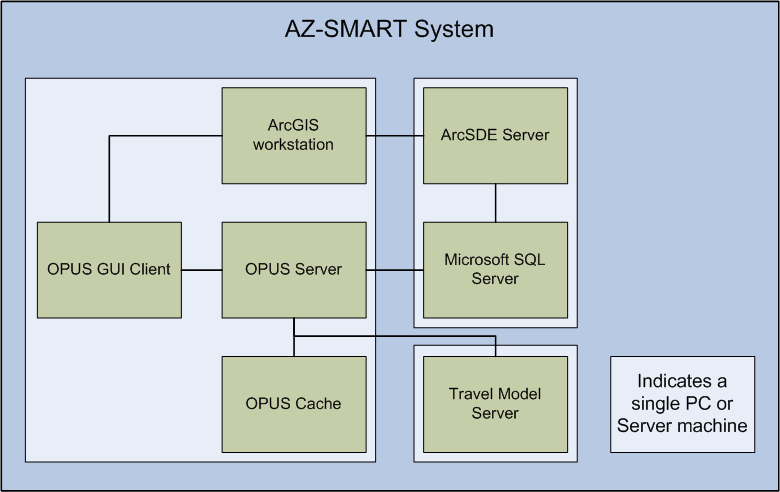
\includegraphics[scale=0.5]{figures/AZ-SMART_system_diagram.png}
\caption{AZ-SMART System Architecture}
\label{figSystem}
\end{center}
\end{figure}
